\documentclass[11pt,letterpaper]{article}
\usepackage[margin=1in]{geometry}
\usepackage[T1]{fontenc}
\usepackage{amsthm}
\usepackage{newtxtext,newtxmath}
\usepackage{microtype,graphicx,booktabs,array,amsmath,enumitem,fancyhdr,xcolor}
\usepackage[colorlinks=true,linkcolor=blue!45!black,urlcolor=blue!45!black,citecolor=blue!45!black]{hyperref}
\usepackage{natbib,xurl,needspace}
\setlength{\emergencystretch}{2em}
\setlength{\parskip}{4pt}
\setlength{\parindent}{14pt}
\setlist{nosep}
\pagestyle{fancy}\fancyhf{}\fancyhead[L]{\small Who Gets to Certify the AI Stack?}\fancyhead[R]{\small Gupta}\fancyfoot[C]{\thepage}\setlength{\headheight}{14pt}
\newtheorem{proposition}{Proposition}
\newcommand{\B}{\mathcal{B}}\newcommand{\Lset}{\mathcal{L}}
\title{Who Gets to Certify the AI Stack?\\\large Authority-Aware Verification and U.S. Alliance Strategy}
\author{Shivam Gupta\\\small Independent Researcher, India and United Arab Emirates\\\small \href{mailto:shivam1720406@gmail.com}{shivam1720406@gmail.com}}
\date{14 October 2026}
\hypersetup{pdftitle={Who Gets to Certify the AI Stack? Authority-Aware Verification and U.S. Alliance Strategy},pdfauthor={Shivam Gupta},pdfsubject={Independent research manuscript}}
\begin{document}
\maketitle
\begin{abstract}
International AI cooperation requires credible verification, but the institutions that certify compliance can also create dependencies. This paper asks when a verification arrangement can reject fabricated approvals while continuing to certify compliant activity after an authority withdraws. It combines an audit of a pinned public GPU-attestation implementation with a finite model separating authority over false approval from authority over service denial. In a constructed two-supplier, two-jurisdiction arrangement, neither an ordinary signature threshold nor nonnegative weighted voting satisfies both requirements, while a Boolean acceptance rule does. If supplier compromise and jurisdictional withdrawal occur together, the same arrangement becomes infeasible; a third independent supplier restores feasibility under the stated assumptions. An exact compiler supplies either an acceptance rule or a concrete impossibility witness. Its implementation agrees with exhaustive Boolean-function checks across 7,371 specifications; 200 structured budget scenarios and 2,000 synthetic dependency assignments test the boundaries. The public-code audit distinguishes local appraisal, vendor-signed reference values, and revocation services without claiming to measure political coercion or deployed hardware security. The contribution is an operational framework for negotiating verification authority in U.S. AI partnerships: independence must be specified for particular claims and failure mechanisms, rather than inferred from the number or location of verifiers.
\end{abstract}
\noindent\textbf{Keywords:} U.S. foreign policy; AI verification; alliances; economic statecraft; remote attestation; general access structures.

\section{Verification as a foreign-policy choice}
The United States faces two connected objectives in international AI policy: encouraging partners to adopt American technology and retaining credible controls over sensitive capabilities. The July 2025 American AI Exports initiative explicitly promoted full-stack packages encompassing hardware, models, infrastructure, cybersecurity, and applications for allies and partners \citep{exports}. These packages make assurance an international institutional question. A partner may operate a data center on its own territory while depending on external organizations to establish that its equipment and software remain acceptable to a buyer or regulator.

This paper examines that dependence at a narrower and more observable boundary than ``AI sovereignty'' in general: the acceptance of a specified verification claim. Who can produce evidence? Who supplies the reference values against which it is judged? Who can revoke an endorsement? Which approvals must the relying party receive? The answers need not identify the same organization, supplier, or jurisdiction. They also need not move together when verification is relocated.

Consider four verification paths arranged across two suppliers and two jurisdictions. A supplier-level compromise can corrupt the paths in one row. A jurisdiction-level withdrawal can disable the paths in one column. Requiring three of four signatures prevents a corrupted row from approving a false claim, but also prevents certification after a column withdraws. Requiring two signatures restores continuity while permitting a corrupted row to approve. Changing the identities that must sign, rather than merely the number, can resolve this conflict. However, that solution fails if compromise and withdrawal must be survived simultaneously. The distinction has consequences for negotiations: a promise that a system is ``redundant'' does not specify which political and technical disruptions it tolerates.

The research question is therefore: \emph{under what explicit allocation of verification authority can an AI partnership retain both false-approval resistance and valid-approval continuity?} Three results answer it. First, a dependency audit can distinguish local execution of a verifier from control of its inputs. Second, a finite separation condition determines whether any monotone acceptance rule can meet a declared pair of threat families. Third, crossing supplier and jurisdiction dependencies can make a typed acceptance rule feasible when every scalar threshold fails; adding a common upstream authority can eliminate that gain.

The paper contributes a policy analysis with an executable institutional-design instrument. It does not introduce threshold signatures, Boolean access structures, correlated-failure analysis, or a new consensus protocol. The mathematical ingredients have established antecedents. The contribution is their explicit application to the allocation of verification authority in U.S. AI partnerships, with a reproducible implementation audit, auditable failure witnesses, and a distinction between alternative and simultaneous disruptions. This is a bounded contribution rather than evidence that an international agreement already has the modeled architecture.

\section{Related research and the boundary of the contribution}
\subsection{Interdependence, certification, and credible partnership}
\citet{farrell} show how network concentration and jurisdiction can enable information gathering and exclusion. The present argument applies that perspective to certification: acceptance of a technical claim can depend on actors other than the facility operator. It adds an operational distinction between the capacity to prevent acceptance and the capacity to make an invalid claim appear acceptable. Those powers can be held by different actors. A shared revocation channel is evidence of a relevant dependency, not evidence that its operator can manufacture any desired device measurement.

The resulting tension is not a choice between complete autonomy and dependence. A U.S. partner may accept external technical expertise while seeking protections against discretionary interruption or unilateral changes in appraisal policy. A supplier may require revocation authority to respond to genuine vulnerabilities. A relying party may refuse continuity arrangements that undermine security. An institutional design has to specify the claims, evidence sources, emergency procedures, and acceptance rules over which these interests operate. No amount of site diversification alone establishes that specification.

\subsection{International AI verification}
\citet{wasil} classify verification methods for unauthorized training and data centers into approaches with different access and hardware requirements. \citet{harack} analyze technical and political feasibility, including mutually verified infrastructure and privacy-preserving computation. \citet{baker} propose six verification layers and discuss supply-chain distrust and allocation of approval authority. These works already recognize that verification mechanisms require protection against abuse and concentration of power. The present paper does not claim discovery of those concerns. It makes a particular design question computable: which combinations of approvals remain distinguishable from fabricated approval coalitions after declared withdrawals?

The narrower scope matters. GPU integrity attestation is not, by itself, verification of a training-compute ceiling, a model's military end use, or the absence of an undeclared data center. An agreement might use hardware attestation as one component, but the agreement's predicate needs an additional measurement and coverage argument. The model below assumes that a noncorrupted verification path correctly tests one shared predicate. Whether that assumption is justified is an empirical and engineering question that must precede its use in policy.

\subsection{General trust and attestation architectures}
Byzantine quorum research has long separated availability and integrity requirements \citep{malkhi}. Asymmetric trust models permit different participants to specify different failure assumptions \citep{alpos2024}. General distributed cryptography implements Boolean access structures and explicitly addresses correlated failure, including locations and software or hardware classes \citep{alpos2023}. Consequently, the inadequacy of node counts under correlated faults is established prior art. Our finite separation result is an elementary access-structure argument, not a new foundational theorem about distributed systems.

RFC 9334 distinguishes attesters, verifiers, relying parties, endorsers, reference-value providers, and policy owners \citep{rats}. Its architecture supplies the vocabulary for mapping technical dependencies. A contemporary industry proposal, OVERT 1.0, also specifies independence of notaries with respect to ownership, infrastructure, and jurisdiction \citep{overt}. Such prescriptions motivate an important question: which independence is necessary for a particular claim? A blanket prohibition on sharing every layer can be unnecessarily expensive, while independence of the final signing organizations can be insufficient if they share the evidence authority.

We use ``authority-aware verification'' for a workflow that records these distinctions and compiles declared assurance requirements into an acceptance rule or failure witness. The name describes an analysis method; it is not a claim to have invented an attestation standard or established a patentable technique. A targeted literature search completed on 14 October 2026 found close work on general trust and AI verification, but no source in the reviewed corpus implementing this exact combined workflow and policy application. That search supports positioning, not a guarantee of universal novelty.

\section{Research design and evidence}
The study has three components with different inferential roles: a public implementation audit, a formal model, and computational verification. Table~\ref{tab:evidence} separates their evidentiary claims. No observed service disruption, political directive, hardware exploit, or international coalition is imputed from a constructed scenario.

\begin{table}[ht]
\centering\small
\begin{tabular}{p{.21\linewidth}p{.35\linewidth}p{.35\linewidth}}
\toprule
Component & Observation or construction & Supported inference \\
\midrule
Public implementation & Seven source files, four configured service defaults, and two root certificates at a pinned revision & Specific code paths and documented allocation of technical roles \\
Boundary execution & Eleven tests of upstream utility functions with synthetic certificates or mocked transport & Behavior of those functions under the declared fixtures \\
Formal model & False-approval sets and honest-live sets for one predicate & Conditional feasibility of an acceptance rule \\
Computational checks & Exhaustive small specifications, structured grids, and seeded synthetic assignments & Agreement with specifications and boundary examples; no population prevalence estimate \\
\bottomrule
\end{tabular}
\caption{Evidence boundaries. The full suite contains 19 tests: 11 upstream-boundary tests and 8 tests of the original compiler and controls.}\label{tab:evidence}
\end{table}

The implementation case is NVIDIA's public \texttt{nvtrust} repository, pinned to revision \nolinkurl{858ada9a17f58c482f578414ea2455498fa51e17}. Selection is purposive: the repository exposes a commercially relevant GPU-attestation stack, local and remote verification options, and code paths for authenticated reference values and certificate status. It is not a representative sample of hardware vendors or confidential-computing products. The source ledger records paths, SHA-256 hashes, line locators, and the extraction procedure. The revision is part of the result; claims about other releases require a new audit.

The documentary corpus comprises the U.S. AI export announcement, the attestation architecture RFC, the vendor's three integration-option pages, its product terms, and the identified research on international AI verification and general trust. It is organized by mechanism rather than by country. Missing legal rights, key-custody arrangements, contractual remedies, and access guarantees remain unknown. Country labels in the model denote constructed withdrawal domains; they are not conclusions about extraterritorial legal reach.

Computational analysis is deterministic except for a separately labeled, seeded synthetic stress corpus. Parameters were fixed to examine small exhaustive specifications, crossed authority structures, shared-authority sensitivity, and simultaneous threats. The synthetic corpus is not fitted to commercial deployments and is not used to estimate their failure frequency. All results and figures are generated from repository scripts. A replication guide distinguishes the solver, the independent truth-table checker, and tests that execute upstream utility functions.

\section{An implementation audit: local verification is a role, not a complete independence claim}
NVIDIA documents three integration forms. Remote verification uses its Remote Attestation Service (NRAS). Local verification performs collection and appraisal locally while using reference-integrity-manifest (RIM) and online-certificate-status (OCSP) services. Customer-managed Trust Outpost caches RIM and OCSP data on premises, subject to appropriate agreements \citep{nremote,nlocal,noutpost}. These are materially different operational arrangements.

Our extractor finds four configurable defaults: GPU and switch NRAS endpoints, a RIM endpoint, and an OCSP endpoint. It also records distinct NVIDIA device-identity and RIM-signing root certificates. The local wrapper passes RIM and OCSP configuration into the verifier; reference manifests may also be supplied through local-file paths. Endpoint replacement therefore changes a delivery path. It does not establish independent authorship of the authenticated material. The claim follows from the pinned source and certificate metadata \citep{nvtrust}; it does not require an inference from the word ``local.''

\begin{table}[ht]
\centering\small
\begin{tabular}{p{.21\linewidth}p{.33\linewidth}p{.36\linewidth}}
\toprule
Technical role & Audited or documented mechanism & Question for a partnership \\
\midrule
Appraisal execution & Remote NRAS or local comparison & Who runs the appraisal, and who may change its policy? \\
Reference values & RIM service or supplied manifest; RIM signing root & Who determines acceptable reference states? \\
Endorsement & Device-identity root certificate & Which authority's statements are relied on? \\
Certificate status & OCSP request and status handling & Which status source and freshness policy are required? \\
Cached delivery & Trust Outpost, described in vendor documentation & How long are cached statements acceptable, and how are updates received? \\
\bottomrule
\end{tabular}
\caption{Technical roles to negotiation questions. Organizational provenance is observable here; a complete legal control map is not.}\label{tab:roles}
\end{table}

To check behavior rather than only names, the suite executes two upstream utility functions. Four tests cover RIM retrieval and HTTP withdrawal at default and overridden URLs. Five OCSP tests use cryptographically signed synthetic responses for good, unknown, key-compromise revocation, and certificate-hold states, including the optional hold exception. Two further tests cover a missing nonce and transport failure. OCSP branch tests stub certificate-chain appraisal and transport; signature verification is executed on the generated responses. These tests do not validate the production certificate chain or run GPU attestation. Their role is to establish the stated boundary behaviors, with all mocking documented in the test source.

The vendor's terms distinguish known-good reference states, signed appraisal reports, certificate status, and caching \citep{nterms}. A cache can reduce dependence on immediate network delivery. Whether it reduces institutional dependence depends on the accepted freshness horizon and on who controls new endorsements and future reference states. For that reason, the audit does not assign the vendor an observed power to falsify a treaty claim. It identifies inputs whose control would have to be examined before declaring verifiers independent.

This distinction supplies the mechanism linking technology to foreign policy. A U.S. export partnership may combine locally hosted compute with an externally governed assurance layer. That architecture could offer useful security expertise and interoperability, but it leaves questions about access, review, and emergency changes. Those questions are conditional institutional implications, not observations that the vendor or U.S. government has exercised coercion through the audited system.

\section{A finite model of certification authority}
\subsection{Claims, authorities, and two forms of disruption}
Let $N=\{1,\ldots,n\}$ index verification paths. Each path returns an authenticated approval of the \emph{same} claim, bound to the same subject, policy version, evidence epoch, and predicate. A signature from another epoch or a different predicate cannot count as a substitute. We consider a fixed relying party with a fixed membership list. The model does not solve consensus between parties, communication scheduling, or membership governance.

A \emph{false-approval family} $\B\subseteq 2^N$ records sets of paths that an allowed capture scenario can cause to approve a false claim. A \emph{live family} $\Lset\subseteq 2^N$ records sets of honest paths guaranteed to approve a valid claim after an allowed disruption. The latter includes timing and freshness requirements through the scenario definition: a path that cannot respond in the agreed window is absent. Both families must be nonempty and explicitly justified.

An authority incidence map can generate these families. If capture of authority $a$ can corrupt path $i$, record that incidence in a capture map. If withdrawal by $a$ can disable $i$, record it in a denial map. An allowed set of authorities induces a union of corrupted paths or a union of disabled paths. The two maps need not coincide. In particular, organizational association alone does not establish a capture edge. It must correspond to an actual ability to falsify the specified predicate or a declared conservative threat assumption.

Initially, capture and denial scenarios are \emph{alternative} tests: false-claim rejection under the capture family, and valid-claim acceptance under the withdrawal family. For simultaneous threats, honest-live sets are replaced by $T\setminus B$ for every allowed pair $(B,T)$. Removing corrupted paths is conservative because a compromised path may withhold its approval of a valid claim. This change is essential; silently treating alternative tests as a joint guarantee overstates resilience.

Let $f:2^N\rightarrow\{0,1\}$ be a monotone acceptance rule. Monotonicity means that adding validly bound approvals cannot turn acceptance into rejection. False-approval resistance requires $f(S)=0$ for every $S\subseteq B$, $B\in\B$. Valid-approval continuity requires $f(T)=1$ for every $T\in\Lset$, and therefore acceptance for any superset. Unlisted failures and false negatives by otherwise honest verifiers lie outside the declared guarantee unless included in these families.

\subsection{Exact feasibility and a reviewable witness}
\begin{proposition}[Finite separation]
A monotone acceptance rule meeting both requirements exists if and only if
\begin{equation}\label{eq:separation}
 T\not\subseteq B\quad\text{for every }T\in\Lset,\ B\in\B.
\end{equation}
If feasible, the rule
\begin{equation}\label{eq:rule}
 f(S)=1\quad\Longleftrightarrow\quad\exists T\in\Lset\text{ with }T\subseteq S
\end{equation}
meets both requirements. If infeasible, a pair $T\subseteq B$ is a concrete failure witness.
\end{proposition}
\begin{proof}
If $T\subseteq B$, continuity requires $f(T)=1$, while false-approval resistance requires $f(T)=0$. Conversely, equation~\eqref{eq:rule} is monotone and accepts every live set. If it accepted a subset of a bad set, some live set would be a subset of that bad set, contradicting equation~\eqref{eq:separation}.
\end{proof}

This is a basic separation argument for general access structures. Its practical value is the witness. A failed negotiation is not reduced to an opaque infeasibility flag: the tool identifies a particular set that has to be accepted for continuity and rejected for integrity. Repair then requires changing the evidence, the dependency map, the allowed disruption family, or the promised guarantee. Renaming organizations or changing a scalar vote threshold cannot resolve the same contradiction.

Only maximal bad sets and minimal live sets need be retained. Removing their redundant subsets and supersets leaves the condition unchanged. The resulting rule is minimally permissive among monotone rules that satisfy the live requirements: it accepts no set whose acceptance is not forced by those requirements. It is not necessarily the smallest Boolean circuit or the least expensive cryptographic implementation. Explicit-family processing and portfolio enumeration can be exponential; the present tool is intended for small, inspectable negotiation models.

For comparison, a scalar rule accepts at least $q$ signatures. Define $b_{\max}=\max_{B\in\B}|B|$ and $\ell_{\min}=\min_{T\in\Lset}|T|$. Its exact feasibility interval is
\begin{equation}\label{eq:threshold}
 b_{\max}<q\leq\ell_{\min}.
\end{equation}
A weighted rule replaces counts with nonnegative weights. It can improve some arrangements, but not all: the crossed example below has an exact impossibility certificate even for arbitrary nonnegative weights.

\subsection{A crossed arrangement that scalar and weighted rules cannot implement}
Let paths be $A_1,A_2,B_1,B_2$, where $A,B$ denote suppliers and subscripts denote jurisdictions (Figure~\ref{fig:cross}). The declared bad sets are supplier rows $\{A_1,A_2\}$ and $\{B_1,B_2\}$. The minimal live sets after either jurisdiction withdraws are the columns $\{A_1,B_1\}$ and $\{A_2,B_2\}$. These are constructed control relationships, not a claim that any current supplier can corrupt these paths.

\begin{figure}[ht]
\centering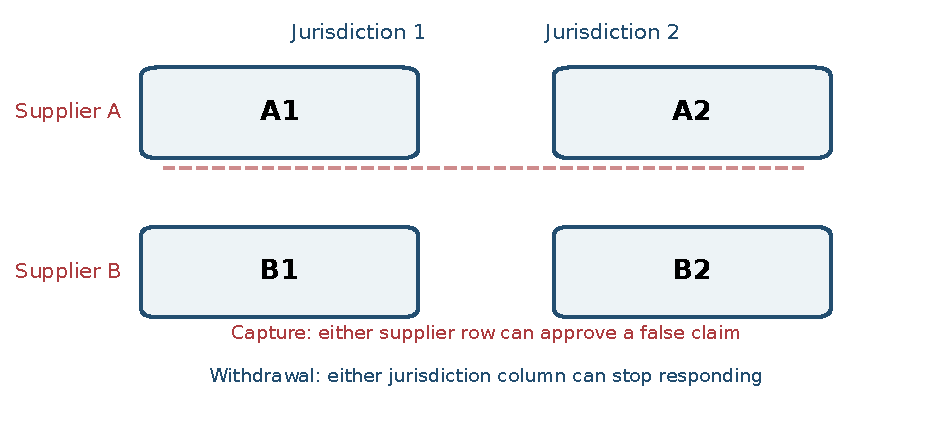
\includegraphics[width=.91\linewidth]{../figures/crossed_authorities.pdf}
\caption{A constructed arrangement separates capture domains (rows) from withdrawal domains (columns). Paths must verify the same predicate. ``Supplier'' independence includes the evidence layer relevant to that predicate, not merely a different company name.}\label{fig:cross}
\end{figure}

Here $b_{\max}=\ell_{\min}=2$, so equation~\eqref{eq:threshold} has no solution. A weighted acceptance threshold $\theta$ would require
\begin{align*}
 w_{A_1}+w_{A_2}&<\theta,&w_{B_1}+w_{B_2}&<\theta,\\
 w_{A_1}+w_{B_1}&\geq\theta,&w_{A_2}+w_{B_2}&\geq\theta.
\end{align*}
Summing the first row gives total weight below $2\theta$; summing the second gives the identical total at least $2\theta$. Thus weighting also fails. A typed rule succeeds:
\begin{equation}\label{eq:typed}
 (A_1\land B_1)\lor(A_2\land B_2).
\end{equation}
The rule accepts a surviving column and rejects either captured row. The symbols describe authenticated approvals, not arbitrary Boolean assertions supplied by the requester. A broader safe rule could accept any pair containing one approval from each supplier; equation~\eqref{eq:typed} is the minimally permissive rule forced by the stated live sets.

\begin{figure}[ht]
\centering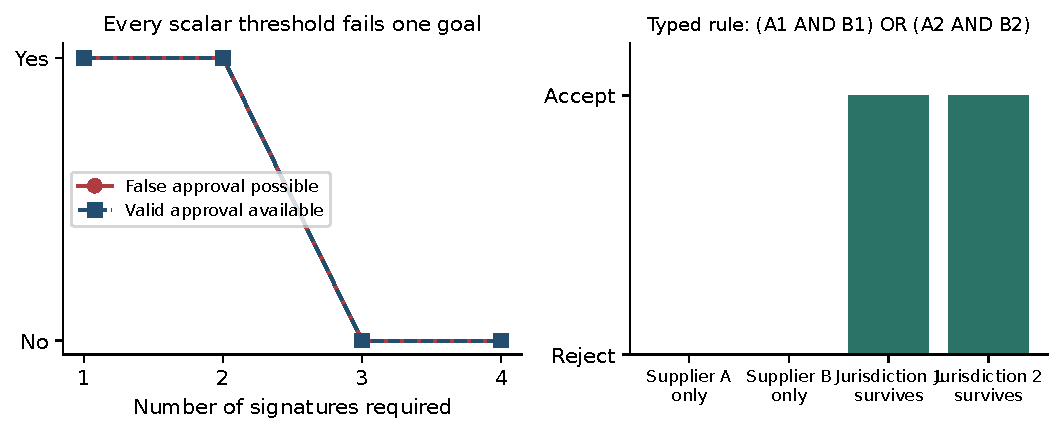
\includegraphics[width=\linewidth]{../figures/rule_comparison.pdf}
\caption{Exact results for the four-path constructed example. In the left panel, thresholds 1 and 2 retain valid approval but permit false approval; thresholds 3 and 4 block both. The right panel evaluates the typed rule on the maximal bad and minimal live sets.}\label{fig:comparison}
\end{figure}

\subsection{Simultaneous threats and a shared-evidence obstruction}
The crossed rule does not survive joint compromise and withdrawal. If supplier $A$ is captured and jurisdiction 2 withdraws, the guaranteed honest-live set is $\{B_1\}$. That set is contained in the bad set arising from capture of supplier $B$. Proposition 1 therefore rules out \emph{every} monotone rule under the enlarged threat family, not merely equation~\eqref{eq:typed}.

More generally, consider a complete grid with $v$ independent supplier rows and $s$ jurisdiction columns. Allow capture of up to $c<v$ suppliers and withdrawal of up to $r<s$ jurisdictions, with no other dependencies. Under alternative tests, a monotone rule exists whenever $v>c$ and $s>r$. Under simultaneous tests, it exists exactly when
\begin{equation}\label{eq:joint}
 v>2c\quad\text{and}\quad s>r.
\end{equation}
Indeed, a simultaneous honest-live set spans $v-c$ suppliers across surviving columns. It is contained in a captured-supplier set exactly when $v-c\leq c$. Otherwise at least one honest-live supplier lies outside any allowed bad set. Scalar rules additionally require
\begin{equation}\label{eq:grid}
 cs<q\leq (v-c)(s-r)
\end{equation}
for simultaneous tests, or $cs<q\leq v(s-r)$ for alternative tests. These expressions count full supplier rows and surviving rectangles; they require the complete-grid and independence assumptions.

For $c=r=1$, three suppliers across two jurisdictions restore simultaneous feasibility. This is a design implication, not a claim that three independent assurance paths for a given GPU predicate are commercially available. Buying another manufacturer's processor does not automatically provide an independent appraisal of the original GPU. Candidate paths must assess the same subject and predicate, potentially through independent measurement mechanisms; replacing the subject changes the research question. If every path instead shares an upstream authority able to falsify that predicate, an allowed capture may give $B=N$. Every nonempty live set is then contained in $B$, making any rule infeasible. If that authority can only interrupt a service, the relevant edge belongs in the denial map; it may still produce an empty live set. The two reasons for failure must not be conflated.

\section{Computational results and falsification checks}
The compiler represents sets as integer bit masks. It reduces the families to antichains, searches for a containment witness, and emits a disjunction of the minimal live sets if no witness exists. A portfolio routine projects both families onto each candidate set of purchased paths and minimizes declared costs. It rejects portfolios that remove a required surviving path. Costs are illustrative units, not market prices or estimated procurement expenditure.

\begin{table}[ht]
\centering\small
\begin{tabular}{p{.47\linewidth}r p{.29\linewidth}}
\toprule
Check & Count & Result \\
\midrule
Exhaustive independent two-authority assignments and budgets & 7,371 & Zero feasibility mismatches \\
Compiled decisions in feasible exhaustive cases & 11,502 & Zero decision mismatches \\
Structured grid/budget/threat-mode scenarios & 200 & Match closed-form conditions \\
Seeded synthetic six-path assignments & 2,000 & 1 scalar-feasible; 60 general-only; 1,939 infeasible \\
Weighted feasible among 60 general-only assignments & 43 & 17 still require a general rule \\
Software tests & 19 & All pass \\
\bottomrule
\end{tabular}
\caption{Computational results. Synthetic category counts describe the fixed generator only. ``General-only'' means feasible for a monotone rule but infeasible for every scalar threshold.}\label{tab:results}
\end{table}

The exhaustive checker enumerates one to three paths, with capture and denial incidences independently assigned to each nonempty subset of two authorities. Both authority budgets range from zero to two. This yields $9(3^2+3^4+3^6)=7,371$ specifications. A separate implementation enumerates every Boolean truth table for each path count, retains only monotone functions, and checks the acceptance and rejection requirements directly. This check does not invoke the compiler to decide feasibility. For feasible cases, it also compares the compiled rule with the direct upward closure of live sets at every signer mask. The 11,502 decision checks and all feasibility checks agree.

Structured scenarios cover $v,s\in\{2,3,4,5\}$, all nontrivial supplier and jurisdiction budgets, and both alternative and simultaneous threats. There are $2(1+2+3+4)^2=200$ such configurations. Compiler outputs agree with equations~\eqref{eq:joint}--\eqref{eq:grid} and their alternative-threat forms. Figure~\ref{fig:grid} shows the scalar interval for the sixteen single-capture, single-withdrawal alternative-threat grids. The four-path case is a boundary where a typed rule changes feasibility. Many larger grids admit scalar rules too; the paper does not claim that typed rules are universally necessary.

\begin{figure}[ht]
\centering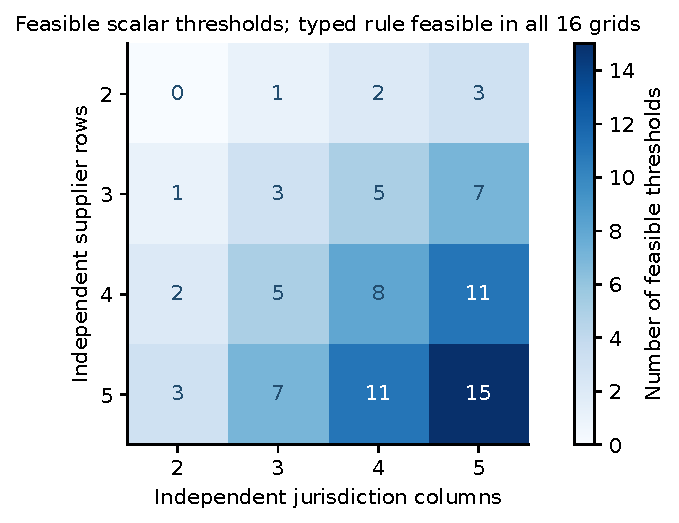
\includegraphics[width=.86\linewidth]{../figures/grid_frontier.pdf}
\caption{Structured scenario analysis under alternative threats: one supplier capture or one jurisdiction withdrawal. Values count feasible scalar thresholds. A general rule is feasible in all 16 grids, including the two-by-two boundary. These are constructed architectures, not observed international arrangements.}\label{fig:grid}
\end{figure}

The synthetic stress corpus uses six paths and five authorities. For each path, the capture subset and denial subset are sampled independently and uniformly from the 31 nonempty authority subsets, using seed 20261014. At most one authority may be captured or withdraw. This deliberately dense incidence generator often creates extensive shared dependencies. It produces 1 scalar-feasible case, 60 cases feasible only with a general rule relative to scalar thresholds, and 1,939 infeasible cases. Linear programs find feasible nonnegative weighted rules for 43 of the 60; the remaining 17 are feasible for general monotone rules but not weighted rules. For all 17 weighted-infeasible cases, the artifact additionally supplies exact rational convex-mixture witnesses: the average incidence vector of bad sets dominates that of live sets in every coordinate, contradicting strict rejection and valid acceptance under any nonnegative weights. The rational sums and inequalities are checked exactly, independently of solver tolerance. These counts are reproducible stress outcomes, not evidence about the prevalence of poor designs in the AI industry.

Several negative controls delimit the result. A common capture authority makes the four-path arrangement infeasible. Simultaneous threats make its original guarantee fail; the six-path, three-supplier arrangement passes under the revised families. Exhaustive portfolio enumeration finds that all four paths are necessary in the canonical alternative-threat example with unit costs, while no portfolio supports a scalar rule. Removing a path does not manufacture resilience by silently removing a threat scenario. The exact weighted contradiction above independently verifies the solver's infeasibility report for the canonical case.

The results are conclusive about the specified model. They do not estimate how likely capture or withdrawal is, demonstrate trustworthy compute metering, or establish that commercial verifiers can implement the required independent paths. Those are distinct claims requiring distinct evidence.

\section{Implications for U.S. foreign policy and commercial assurance}
\subsection{Negotiate the assurance layer of the exported stack}
The American AI Exports initiative creates a concrete policy setting for these questions. An exported stack can include technically sound assurance while retaining concentrated control over its acceptance. U.S. negotiators should therefore distinguish three commitments: access to compute, access to verification inputs, and recognition of verification results. A partner can possess the first without autonomous control over the other two. The model identifies which acceptance dependencies matter to a specified assurance promise.

A practical bilateral or plurilateral schedule could define the verified predicate, evidence identifiers, appraisal-policy owner, membership authority, and permitted continuity rule. Each claimed independent path would disclose its capture and denial dependencies, including upstream endorsements and reference-value sources. The schedule would specify whether its guarantee covers alternative disruptions or simultaneous ones. A failure witness would expose an unresolved institutional conflict before it becomes a disagreement during an interruption.

This recommendation does not imply bypassing U.S. export controls or removing security revocation. The 2025 AI Diffusion Rule's announced rescission illustrates that the governing policy framework can change \citep{bis}; the present analysis is not a statement of current licensing requirements. Any continuity commitment would need a lawful scope, security exceptions, and an agreed process for challenging the exception. A certificate whose issuer legitimately revokes it after compromise cannot be restored to validity by a favorable voting rule. The modeled guarantee applies only when its predicate and honest-verifier assumptions remain justified.

\subsection{Preserve technical denial while limiting discretionary dependence}
U.S. policy can have reasons to retain the ability to deny sensitive capability to prohibited recipients. Partners can have reasons to resist unrelated unilateral interruption of agreed uses. These objectives concern different classes of decisions. A durable arrangement would document security-critical predicates and their revocation procedures separately from changes in commercial access or political recognition. The mathematical model does not choose the appropriate boundary, but it makes the consequences of a proposed boundary inspectable.

This suggests a specific institutional hypothesis: partners will find an assurance arrangement more credible when its declared independence reaches the layer controlling the claim, and when exceptional refusal is attributable and reviewable. The study does not test whether such provisions increase adoption, investment, or alliance cohesion. Those are follow-on empirical questions. The causal chain proposed here is architectural dependency, potential certification bottleneck, bargaining over exceptional authority, and finally possible effects on partnership choices. Only the first link is audited; the middle links are modeled and the final link remains a hypothesis.

A partner-operated verifier can provide meaningful agency over appraisal execution and policy even while continuing to rely on supplier endorsements. That agency should be described precisely rather than dismissed as illusory or advertised as complete independence. A U.S.-led arrangement may be strengthened by this division of authority if partners can reproduce appraisals, inspect changes, and exercise agreed review rights. The relevant policy choice is an allocation of roles with explicit limits, not an undifferentiated transfer of all technical control.

\subsection{Design for simultaneous emergencies when the commitment requires it}
An assurance label covering supplier compromise and another covering jurisdictional continuity do not automatically compose. The four-path example passes each alternative test but fails their joint requirement. If a foreign-policy commitment promises continuity during a crisis in which both are plausible, the joint family belongs in the contract. Conversely, if simultaneous threats are outside the commitment, that limitation should be visible to the relying party.

The model also reveals the cost of overbroad independence requirements. Some arrangements admit scalar rules; others benefit from identifying which actors signed. Procurement should compare explicit feasible portfolios rather than maximize the count of logos, regions, or signatures. The tool's failure witness can distinguish a shortage of independent evidence from a poorly chosen acceptance rule. The former requires institutional or technical investment; the latter may be repairable without buying another verification path.

\subsection{A bounded commercial opportunity}
There is a plausible commercial application in assurance design and procurement review. A software service could ingest a verified dependency ledger, a customer's allowed threat families, and candidate verification costs; then produce a signer rule, minimal failure witnesses, and portfolio comparisons. It could monitor changes in endorsements, policies, membership, and recognized evidence epochs that invalidate an earlier design analysis. The present repository implements the finite compiler and portfolio calculation, not automated legal analysis, vendor integration, or a commercial product.

Demand is plausible because publicly documented attestation systems already offer multiple deployment forms and configurable service endpoints. Nevertheless, no customer interviews, willingness-to-pay measurements, market-size estimate, or patentability opinion is supplied. Originality of a policy application is also not evidence of patent novelty. The defensible product value would be maintained dependency evidence and reviewable institutional assurance, built on established cryptographic primitives and general trust analysis.

\section{Limitations and a falsifiable research agenda}
The implementation audit is one purposively chosen case. It cannot establish a market-wide pattern, and it does not inspect private contracts or key-management systems. Configurable URLs, cached data, and certificate organization fields do not settle the legal scope of a government's authority. A deployment could have additional protections or dependencies absent from the reviewed public code. These unknowns must be resolved before attaching a production assurance claim to the model.

The formal model assumes a fixed, agreed predicate and correctly bound approvals. It does not address contradictory national definitions of compliance, leakage from inspection, the accuracy of measurement hardware, undisclosed compute, or retaliation after a verifier refuses. It treats authority capture and withdrawal sets as inputs rather than estimating them. Real authorities can exert partial, probabilistic, or time-dependent influence; a conservative finite family is an abstraction that needs justification.

Monotone acceptance is appropriate for a fixed epoch with authenticated signer identity and nonconflicting approvals. If a protocol requires rejection when additional evidence reveals a contradiction, the approval-only abstraction is insufficient. Such a system needs signed negative findings and evidence reconciliation before this model is applied. Similarly, membership rotation must be governed independently: a common registrar able to replace trusted signers is a possible capture dependency, not an implementation detail that can be omitted.

Four observations would change the practical interpretation. First, a deployment with independent evidence acquisition and independently governed reference approval could falsify an assumed common capture edge. Second, an offline arrangement with an agreed validity horizon could eliminate a particular immediate denial edge. Third, a legal or technical rule requiring universal participation could constrain the permitted acceptance functions and invalidate the apparent benefit of a typed rule. Fourth, inability to bind approvals to a shared predicate would invalidate the voting model altogether. The repository makes each edge and family explicit so these revisions can be tested instead of absorbed into an ambiguous resilience score.

\Needspace{8\baselineskip}
\section{Conclusion}
AI verification infrastructure is a prospective site of international authority as well as a security technology. Its relevant dependencies extend beyond the location of computation or the number of final signers. A policy commitment must specify who can make a false approval possible, who can prevent a valid approval, and whether those events must be survived together.

The public implementation audit establishes a concrete distinction between appraisal execution and externally authored inputs. The finite model then shows when a declared assurance promise is implementable, when a typed acceptance rule repairs a scalar-voting limitation, and when no rule can repair a common upstream dependency. For U.S. AI partnerships, the practical contribution is a reviewable way to negotiate and test certification authority before promising independence or continuity. The strength of the conclusion lies in its explicit scope: assurance follows from claim-specific dependencies and a declared threat family, rather than from an architectural label.

\paragraph{Code and data availability.} Original scripts, derived results, tests, figures, evidence ledger, and manuscript sources are available at \url{https://github.com/shi1720/authority-aware-assurance}. Third-party code is fetched at the pinned revision by the replication script and remains subject to its own license. No third-party source is silently substituted after an upstream update.
\paragraph{Author and competing interests.} Shivam Gupta is an independent researcher and founder of Siloed, a software consultancy. The commercial application discussed here is prospective; the paper reports no evaluation of a consultancy client and attributes no vendor or government sponsorship.

\begin{thebibliography}{99}
\bibitem[Alpos and Cachin(2023)]{alpos2023} Alpos, Orestis, and Christian Cachin. 2023. Do Not Trust in Numbers: Practical Distributed Cryptography With General Trust. \emph{Stabilization, Safety, and Security of Distributed Systems}. \href{https://doi.org/10.1007/978-3-031-44274-2_40}{doi:10.1007/978-3-031-44274-2\_40}. Open version: \url{https://eprint.iacr.org/2022/1767}.
\bibitem[Alpos et~al.(2024)]{alpos2024} Alpos, Orestis, Christian Cachin, Bj\"orn Tackmann, and Luca Zanolini. 2024. Asymmetric distributed trust. \emph{Distributed Computing} 37:247--277. \href{https://doi.org/10.1007/s00446-024-00469-1}{doi:10.1007/s00446-024-00469-1}.
\bibitem[Baker et~al.(2025)]{baker} Baker, Mauricio, Gabriel Kulp, Oliver Marks, Miles Brundage, and Lennart Heim. 2025. Verifying International Agreements on AI: Six Layers of Verification for Rules on Large-Scale AI Development and Deployment. RAND report WR-A4077-1. \url{https://arxiv.org/abs/2507.15916}.
\bibitem[BIS(2025)]{bis} Bureau of Industry and Security. 2025. Department of Commerce Announces Rescission of Biden-Era Artificial Intelligence Diffusion Rule, Strengthens Chip-Related Export Controls. May 13. \url{https://media.bis.gov/press-release/department-commerce-announces-rescission-biden-era-artificial-intelligence-diffusion-rule-strengthens}.
\bibitem[Farrell and Newman(2019)]{farrell} Farrell, Henry, and Abraham L. Newman. 2019. Weaponized Interdependence: How Global Economic Networks Shape State Coercion. \emph{International Security} 44(1):42--79. \href{https://doi.org/10.1162/isec_a_00351}{doi:10.1162/isec\_a\_00351}.
\bibitem[GLACIS Technologies(2026)]{overt} GLACIS Technologies. 2026. \emph{OVERT 1.0---Open Standard}. March. ATT-5.3, p. 44. Industry proposal, not an IETF or government standard. \url{https://overt.is/OVERT_v1.0_STANDARD.pdf}.
\bibitem[Harack et~al.(2025)]{harack} Harack, Ben, Robert F. Trager, Anka Reuel, David Manheim, Miles Brundage, et al. 2025. Verification for International AI Governance. Oxford Martin AI Governance Initiative. July 3. \url{https://aigi.ox.ac.uk/publications/verification-for-international-ai-governance/}.
\bibitem[IETF(2023)]{rats} Birkholz, Henk, Dave Thaler, Michael Richardson, Ned Smith, and Wei Pan. 2023. Remote ATtestation procedureS (RATS) Architecture. RFC 9334. \href{https://doi.org/10.17487/RFC9334}{doi:10.17487/RFC9334}. \url{https://www.rfc-editor.org/rfc/rfc9334.html}.
\bibitem[Malkhi and Reiter(1998)]{malkhi} Malkhi, Dahlia, and Michael Reiter. 1998. Byzantine quorum systems. \emph{Distributed Computing} 11:203--213. \href{https://doi.org/10.1007/s004460050050}{doi:10.1007/s004460050050}.
\bibitem[NVIDIA(2026a)]{nvtrust} NVIDIA. 2026a. \emph{nvtrust: Ancillary open source software to support confidential computing on NVIDIA GPUs}. Revision \nolinkurl{858ada9a17f58c482f578414ea2455498fa51e17}. \url{https://github.com/NVIDIA/nvtrust/tree/858ada9a17f58c482f578414ea2455498fa51e17}.
\bibitem[NVIDIA(2026b)]{nlocal} NVIDIA. 2026b. Attestation using Local Verifier. Documentation, updated October 6. \url{https://docs.nvidia.com/attestation/poc-to-production/latest/integration-options/local_verifier.html}.
\bibitem[NVIDIA(2026c)]{nremote} NVIDIA. 2026c. Attestation using NRAS. Documentation. \url{https://docs.nvidia.com/attestation/poc-to-production/latest/integration-options/remote_verifier.html}.
\bibitem[NVIDIA(2026d)]{noutpost} NVIDIA. 2026d. Customer-Managed Attestation. Documentation, updated October 6. \url{https://docs.nvidia.com/attestation/poc-to-production/latest/integration-options/trust_outpost.html}.
\bibitem[NVIDIA(2026e)]{nterms} NVIDIA. 2026e. Product-Specific Terms for Confidential Computing. Current web version, accessed October 14. \url{https://www.nvidia.com/en-us/agreements/enterprise-software/product-specific-terms-for-confidential-computing/}.
\bibitem[Wasil et~al.(2024)]{wasil} Wasil, Akash R., Tom Reed, Jack William Miller, and Peter Barnett. 2024. Verification methods for international AI agreements. \url{https://arxiv.org/abs/2408.16074}.
\bibitem[White House(2025)]{exports} White House. 2025. Fact Sheet: President Donald J. Trump Promotes the Export of American AI Technologies. July 23. \url{https://www.whitehouse.gov/fact-sheets/2025/07/fact-sheet-president-donald-j-trump-promotes-the-export-of-american-ai-technologies/}.
\end{thebibliography}

\appendix
\section{Executable specification and replication}
A compact version of the acceptance calculation is:
\begin{verbatim}
def compile_rule(bad, live):
    for surviving in live:
        for fabricated in bad:
            if surviving <= fabricated:
                return {"feasible": False,
                        "witness": (surviving, fabricated)}
    return {"feasible": True, "clauses": minimal_sets(live)}

def accept(clauses, approvals):
    return any(clause <= approvals for clause in clauses)
\end{verbatim}
Here sets are mathematical sets; the repository uses equivalent integer bit masks and includes antichain reduction. Signature authentication, predicate binding, identity validation, and freshness are prerequisites outside this compiler. The compiler does not transform an untrusted claim into trustworthy evidence.

For weighted rules the solver imposes a unit rejection margin, $\sum_{i\in B}w_i-\theta\leq-1$, and acceptance constraints $\theta-\sum_{i\in T}w_i\leq0$, with nonnegative weights. On a finite family any strict feasible separation can be scaled to a unit margin. Solver results are checked against every input constraint. Weighted infeasibility certificates give probability mixtures of bad and live sets whose expected incidence vectors satisfy $E[B]\geq E[T]$ coordinatewise. For nonnegative weights this implies $E[w(B)]\geq E[w(T)]$, contradicting $w(B)<\theta\leq w(T)$. Mixture coefficients are converted to rational numbers and checked exactly; every reported weighted-infeasible synthetic case has such a certificate. The canonical infeasibility is also established by the exact summed-inequality argument in the main text.

The artifact requires Python 3.12 and includes a version-pinned dependency lock. From its root:
\begin{verbatim}
python -m venv .venv
.venv/bin/pip install -r requirements.lock
.venv/bin/python src/fetch_upstream.py work/nvtrust
.venv/bin/python src/audit_upstream.py work/nvtrust
NVTRUST_SOURCE="$PWD/work/nvtrust" \
  .venv/bin/python -m pytest tests -q
.venv/bin/python src/experiments.py
.venv/bin/python src/figures.py
cd paper && tectonic manuscript.tex
\end{verbatim}
The checkout is obtained from the vendor repository at an exact commit. Hash checks verify seven audited source files and two certificates. The boundary tests replace transport and, where documented, certificate-chain appraisal. They require no device or vendor account. The experiment checker enumerates truth tables independently of the compiler; the synthetic generator and all classifications are saved in JSON. Reproduction makes no paid API requests.

\section{An assurance schedule for a proposed partnership}
A reviewable assurance schedule would contain the following fields, each attached to evidence or marked unresolved:
\begin{enumerate}
\item \textbf{Claim binding:} subject identifiers, predicate, policy version, evidence epoch, signer identities, and accepted response window.
\item \textbf{Technical roles:} collector, appraiser, reference-value provider, endorser, status provider, and relying-party policy owner.
\item \textbf{Control maps:} documented capture and denial incidences, distinguishing confirmed capabilities from conservative stress assumptions.
\item \textbf{Threat family:} allowed authority combinations, whether capture and withdrawal occur alternatively or simultaneously, and the treatment of honest-verifier disagreement.
\item \textbf{Result:} acceptance rule or impossibility witness, and the specific changes required to repair the latter.
\item \textbf{Governance changes:} membership rotation, key replacement, policy updates, security revocation, attribution, review, and revalidation obligations.
\end{enumerate}
\end{document}
